\documentclass[journal]{IEEEtran}

\usepackage{graphicx}
\usepackage{url}
\begin{document}

\title{Enhanced Multi-Robot Coordination Utilizing ChatGPT: Design Principles and Experimental Investigation}

\author{Baran~Arig,
        Varun~Iyengar,
       Shanmukha~Rao~Allipilli
\thanks{Baran Arig, Varun Iyengar, and Shanmukha Rao Allipilli are with the Department of Electrical and Computer Engineering, Drexel University, Philadelphia, USA. (e-mail: ba646@drexel.edu, vi44@drexel.edu, sa3935@drexel.edu)}
\thanks{Also special thanks to Professor Lifeng Zhou for his guidance and support throughout this project Dr. Lifeng Zhou is with the Department of Electrical and Computer Engineering, Drexel University, Philadelphia, USA. (e-mail: lz457@drexel.edu)}
}

\maketitle

\begin{abstract}
In this paper, we present an enhanced version of ChatGPT tailored for multi-robot coordination tasks, specifically in scenarios involving the coordination of multiple drones for object surveillance. Leveraging the capabilities of ChatGPT, we address the challenges inherent in orchestrating a team of autonomous agents to collaboratively survey an object of interest. We elucidate the design principles behind the integration of ChatGPT into the multi-robot system and explore its performance through experimental investigation. Our results demonstrate the efficacy of the proposed approach in facilitating efficient communication and coordination among the robotic agents, thereby improving the overall task performance in multi-robot environments. 
\end{abstract}

\begin{IEEEkeywords}
ChatGPT, multi-robot coordination, object surveillance, communication, coordination, robotics.
\end{IEEEkeywords}

\section{Introduction}
\IEEEPARstart{T}{he} utilization of robotic systems for various applications has surged in recent years, encompassing domains such as surveillance, search and rescue, and environmental monitoring. In many of these applications, the deployment of multiple robots offers distinct advantages over single-agent systems, including increased coverage, redundancy, and task parallelism. However, effective coordination among these autonomous agents remains a fundamental challenge. 

In previous work [1], we did a basic implementation of the ChatGPT for Robotics paper. ChatGPT is a state-of-the-art conversational AI model developed by OpenAI. While our initial investigation focused on the application of ChatGPT in single-robot scenarios, in this paper, we extend our study to encompass multi-robot environments, particularly in the context of coordinating multiple drones for object surveillance tasks.

The extension of ChatGPT to multi-robot coordination introduces several novel challenges and opportunities. Unlike single-agent settings, where the focus is primarily on human-robot interaction, multi-robot systems entail intricate coordination and communication mechanisms among the robotic agents themselves. Consequently, the integration of ChatGPT into such environments necessitates careful consideration of design principles tailored to facilitate seamless communication and collaboration among the robots.

In this paper, we present an expanded version of our previous work, wherein we augment the parameters and features given to ChatGPT to enable effective communication and coordination in multi-robot environments, the environment being used here is Microsoft Airsim. We delineate the design principles underpinning the integration of ChatGPT into the multi-robot system architecture, emphasizing the unique challenges posed by the coordination of drones for object surveillance. Furthermore, we conduct extensive experimental evaluations to assess the performance of the proposed approach in real-world scenarios, validating its efficacy in enhancing multi-robot coordination capabilities.

The remainder of this paper is organized as follows. Section II provides a brief overview of related work in the field of multi-robot coordination and communication. Section III describes the implementation to get the system to work. Section IV delineates the design principles guiding the integration of ChatGPT into the multi-robot system architecture, Airsim. Section V presents the experimental setup and methodology employed to evaluate the proposed approach. Section VI discusses the experimental results and analyzes the performance of the system. Section VII mentions the Potential Future Impact. Finally, Section VIII concludes the paper with a summary of findings and outlines directions for future research.




\section{Related Work}

The emergence of conversational AI models, such as ChatGPT, has sparked significant interest in their application to a wide array of topics, one of them being robotics. One notable work in this domain is the ChatGPT for robotics paper by Vemprala et al. [1]. In this paper, the authors introduce ChatGPT as a versatile tool for human-robot interaction and task assistance. The model is specifically tailored to address the challenges of natural language understanding and generation in robotic systems.

Vemprala et al. showcase the capabilities of ChatGPT in various robotics applications, including but not limited to object manipulation, navigation, and assistance tasks. They highlight the model's ability to understand and respond to human commands and queries in real-time, enabling seamless interaction between humans and robots.

Of particular relevance to our work is the exploration of ChatGPT's potential in multi-robot environments. While the initial focus of the paper is on single-agent scenarios, the authors hint at the adaptability of ChatGPT to coordinate multiple robots effectively. However, further investigation into the integration of ChatGPT into multi-robot systems is warranted, particularly in complex tasks such as object surveillance with multiple drones.

Building upon the insights provided by Vemprala et al., we extend the applicability of ChatGPT to multi-robot coordination, with a specific emphasis on coordinating drones for object surveillance tasks. By leveraging the principles outlined in their work, we augment the instructions fed to ChatGPT to facilitate seamless communication and collaboration among multiple robotic agents, thereby enabling he multi-robot system.

\section{Implementation}

In this section, we detail the implementation of the proposed methodologies for leveraging OpenAI's ChatGPT in robotics applications. Our approach is based on a systematic pipeline that combines prompt engineering, function library design, context description, and task-specific prompting strategies to enable ChatGPT to effectively reason and execute a variety of robotics tasks.
We begin by defining a high-level robot function library tailored to the specific form factor or scenario of interest. This library comprises descriptive function names mapped to actual implementations from existing libraries. For instance, functions like detectObject(objectName) and moveTo(x, y, z) are defined, which internally link to relevant OpenCV or motion planning implementations. The function names are designed to be descriptive enough that ChatGPT can follow and decipher their intended function with ease.  Clear and concise names facilitate LLMs to reason over functional connections between APIs, thereby producing the desired outcomes for the given problem. Listing such high-level functions in the prompt facilitates ChatGPT in creating logical sequences of behavioral primitives and ensures generalization across different scenarios and platforms. It is recommended to provide explanations of APIs and, if necessary, break them down into sub-components with clear inputs and outputs akin to code documentation. Further ahead we have an example prompt input which details multiple functions, their inputs, and what is expected when the function runs. This approach aids ChatGPT in understanding the functionalities of APIs comprehensively, facilitating accurate reasoning and execution. The flexibility of LLMs to define new functions lends great competency to LLMs in addressing various challenges encountered in robotics applications.

A crucial aspect of our implementation is providing clear and concise context descriptions along with task-specific prompts to guide ChatGPT's reasoning. These descriptions encompass constraints, environment details, current state, goals, objectives, and solution examples. By specifying relevant information such as object properties, environment characteristics, and desired outcomes, we ensure that ChatGPT generates accurate and contextually relevant responses. This includes context like details about a maze being traversed, the number of pieces that need to be assembled in a puzzle, or how similar tasks can be solved. Good prompting practice defines a plethora of functions for the robot's functions and tasks are specifically stated. If the initial prompt the user sends is not enough to complete the task at hand, the user is involved in the loop to continue the conversation with ChatGPT and input more information to aid with the task. This usually ends up in the LLM providing an output in the form of first a block of descriptive text and then a related code block. This is done with OpenAI’s Codex model which is specifically tailored for code generation tasks. This model is prompted through the use of forcing the LLM to respond in a certain fashion like providing python or C++ code.

\begin{figure}[h]
    \centering
    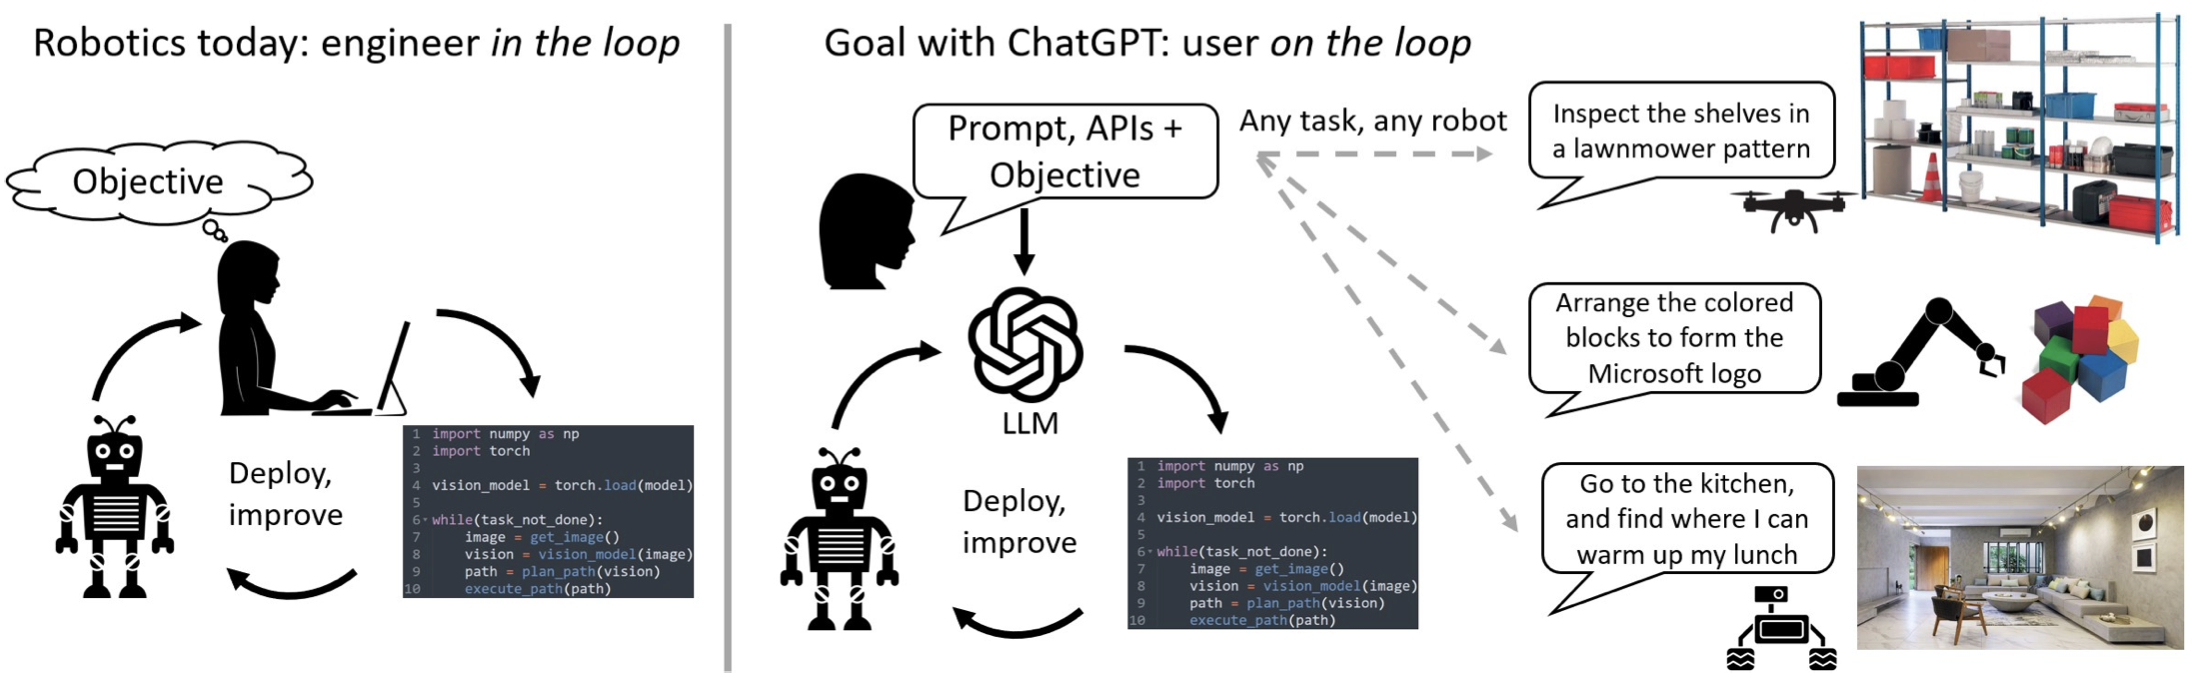
\includegraphics[width=1\linewidth]{img1.png}
    
    
\end{figure}
This image from the referenced paper is a great example of what we mean, with the user not actively programming a solution but still heavily involved in the design and control process through their conversation with the LLM.


We simulated a scenario where we control two robots to move from their launchpad over to a blue car, hover over the car, and return and land back on the launchpad. The user provides instructions in natural language, and ChatGPT interprets and executes the commands accordingly. It took multiple commands from the user to complete this scenario as we needed to launch the drones and move them to and from a destination. Each of these steps took two commands as each drone was moved separately. This simulator is what we focused on in our implementation of the project, aiming to control multiple robots beyond the singular drone highlighted in most of the referenced paper. This required multiple updates to be able to implement the multi-robot schema. The biggest of which were in the settings.json file which held the setup for the simulator, the prompt text for ChatGPT to start off with,and the Airsim wrapper file itself. In the settings file we defined two drones offset by 2 units in the y axis so they generate in a line on the helipad. The camera for the simulator was attached to drone 1 so drone 1 was only in visible when near drone 1 or inside the cone of vision specified in the settings file. In the following image of the prompt text file you see the specifications of the functions being defined. 
\begin{figure}[h]
    \centering
    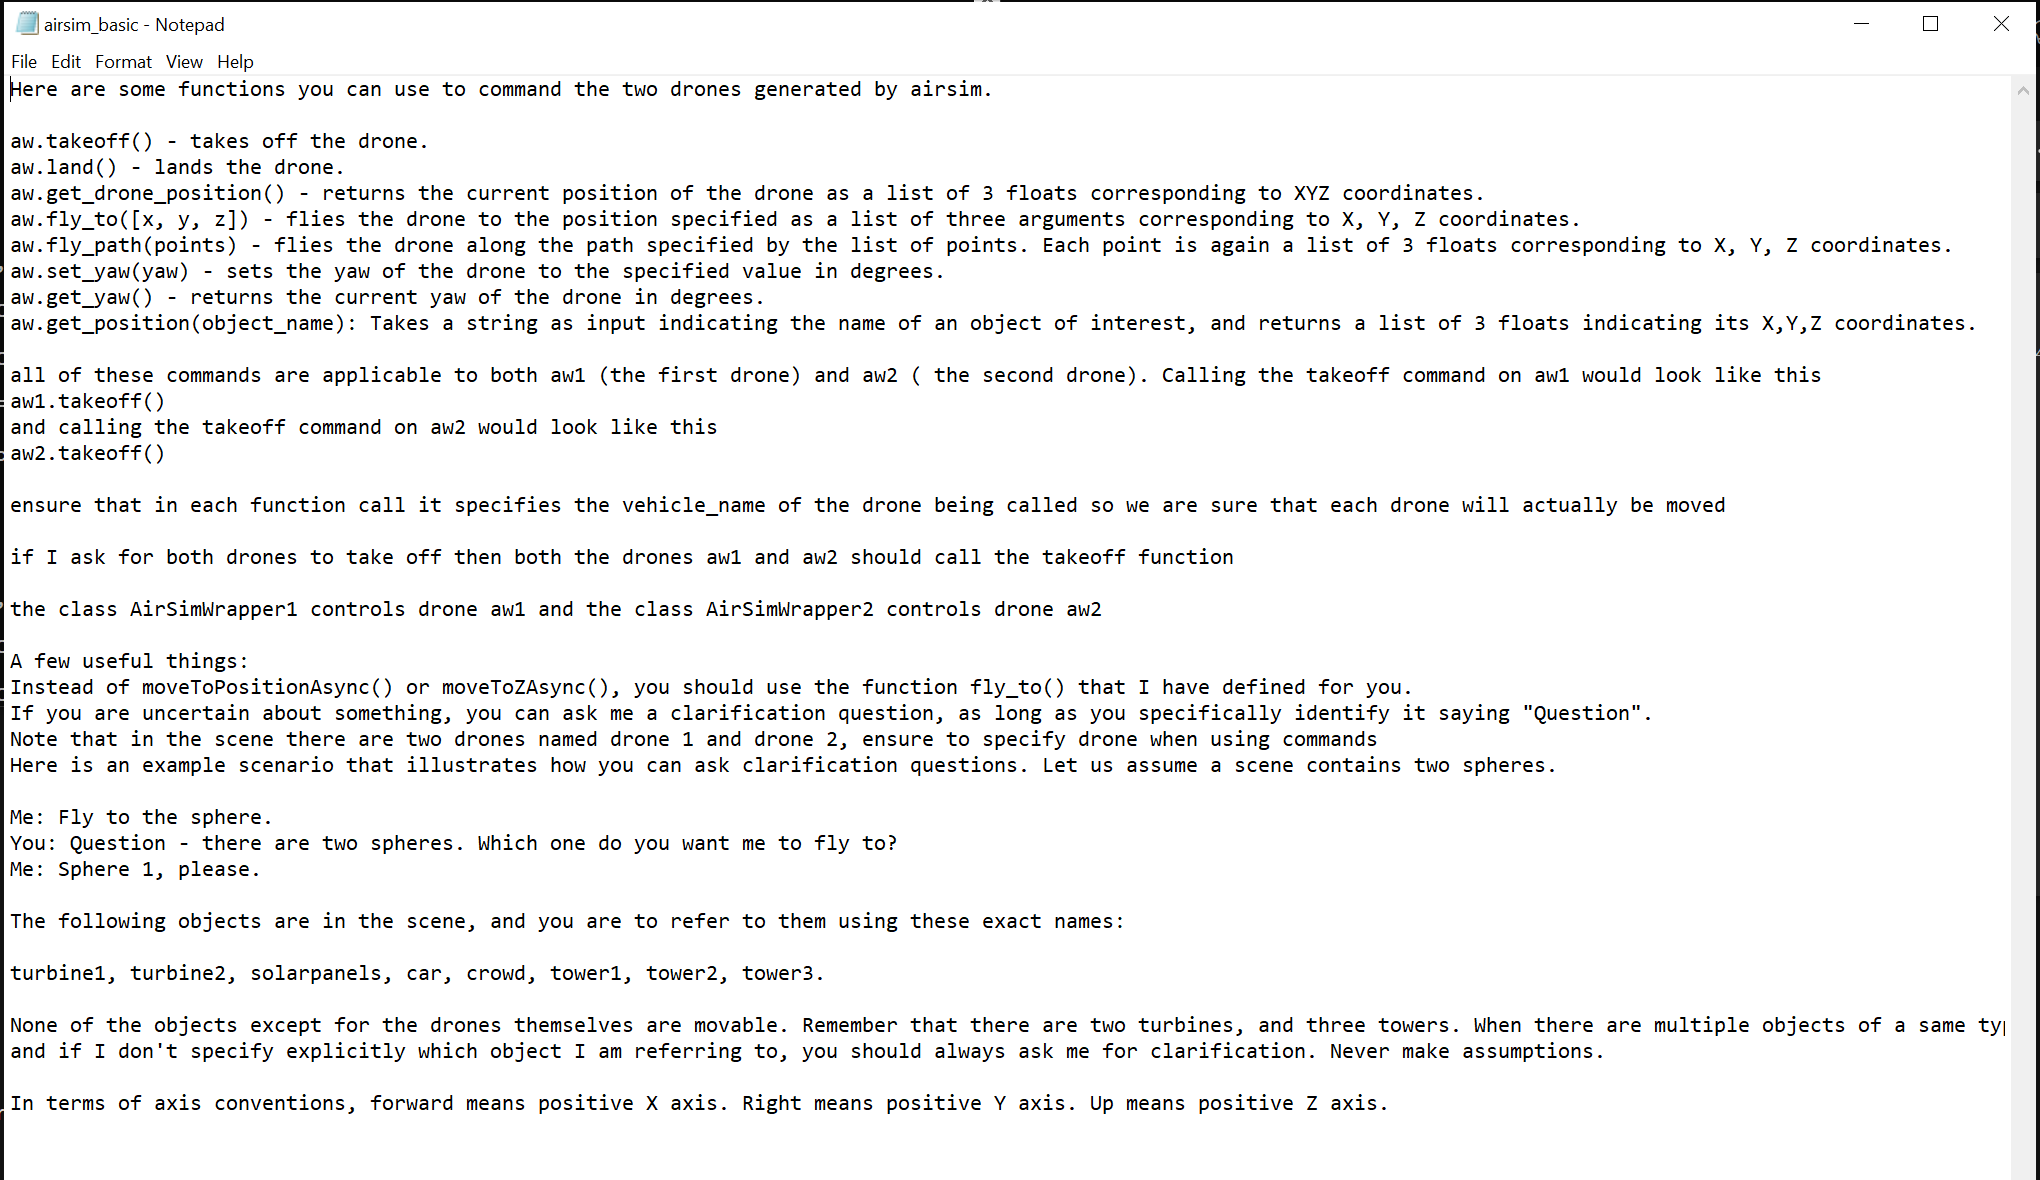
\includegraphics[width=1\linewidth]{prompt.PNG}
    \caption{Enter Caption}
    \label{fig:enter-label}
\end{figure}
As stated above these function definitions need to be precise and the name must be clear to understand the design of the function. It also specifies we are using two drones, each drone needs to be controlled separately, and what to refer to each drone as. This is done for ease of use of the functions, being able to use the vehicle name defined in the settings file to refer to each drone separately. This vehicle naming scheme does provide a small issue when it comes to scalability of the code. Each vehicle name now needs to be hardcoded into the repository to ensure each vehicle is being initialized and called properly[2]. This implies that the individual who sets up multi robot environments would need to be technical enough to grasp those concepts, which could further narrow the region in which a non technical person is able to interact in this fashion.

In the above prompt we also present examples of a conversation held between the user and ChatGPT so it can respond properly and accurately gather data from the user. The prompt also defines some objects in the area for ease of access so they can be used and landmarks for movement. Once again the aim of this is for everything to be as accurate and clear as possible to remove any chance of confusion from ChatGPT as to exactly what the user wants.

The utilization of Microsoft AirSim for simulating robotics scenarios demonstrates the versatility and adaptability of ChatGPT in virtual environments. By accurately parsing user instructions and generating corresponding control commands, ChatGPT showcases its potential for assisting in various robotics applications, including industrial inspections and aerial surveillance.
\section{Design Principles for Multi-Robot Coordination}

 The design principles guiding the integration of ChatGPT into a multi-robot coordination system tailored for object surveillance tasks.

A. Decentralized Communication Architecture: Given the distributed nature of multi-robot systems, we design a decentralized communication architecture to enable seamless interaction among the drones. Each drone acts as both a communicator and a decision-maker, leveraging ChatGPT for natural language understanding and generation. This architecture minimizes communication overhead and enhances robustness by allowing drones to adapt to dynamic environmental changes autonomously.

B. Adaptive Task Allocation Strategies: Efficient task allocation is critical for optimizing the coverage area and minimizing redundant efforts in object surveillance tasks. We employ adaptive task allocation strategies that leverage ChatGPT's contextual understanding to dynamically assign surveillance regions to individual drones based on factors such as object importance, environmental conditions, and agent capabilities. These strategies ensure optimal resource utilization and enhance the overall effectiveness of the surveillance mission.

C. Context-aware Decision Making: To enable context-aware decision making, we integrate ChatGPT into the decision-making process of each drone. By contextualizing the information gathered from sensors with natural language inputs, drones can make informed decisions regarding movement, observation angles, and object tracking. This integration enhances the adaptability and intelligence of the multi-robot system, allowing it to respond effectively to dynamic changes in the surveillance environment.
...
\section{Experimental Evaluation}

 The experimental methodology used to evaluate the performance of the ChatGPT-integrated multi-robot coordination system for object surveillance tasks.

A. Simulation Environment: We employ a realistic simulation environment that simulates various surveillance scenarios, including urban environments, wilderness areas, and indoor spaces. The environment incorporates dynamic objects, obstacles, and environmental conditions to mimic real-world surveillance missions accurately. This enables us to evaluate the system's performance under diverse conditions and assess its robustness and scalability.
\begin{figure}[h]
    \centering
    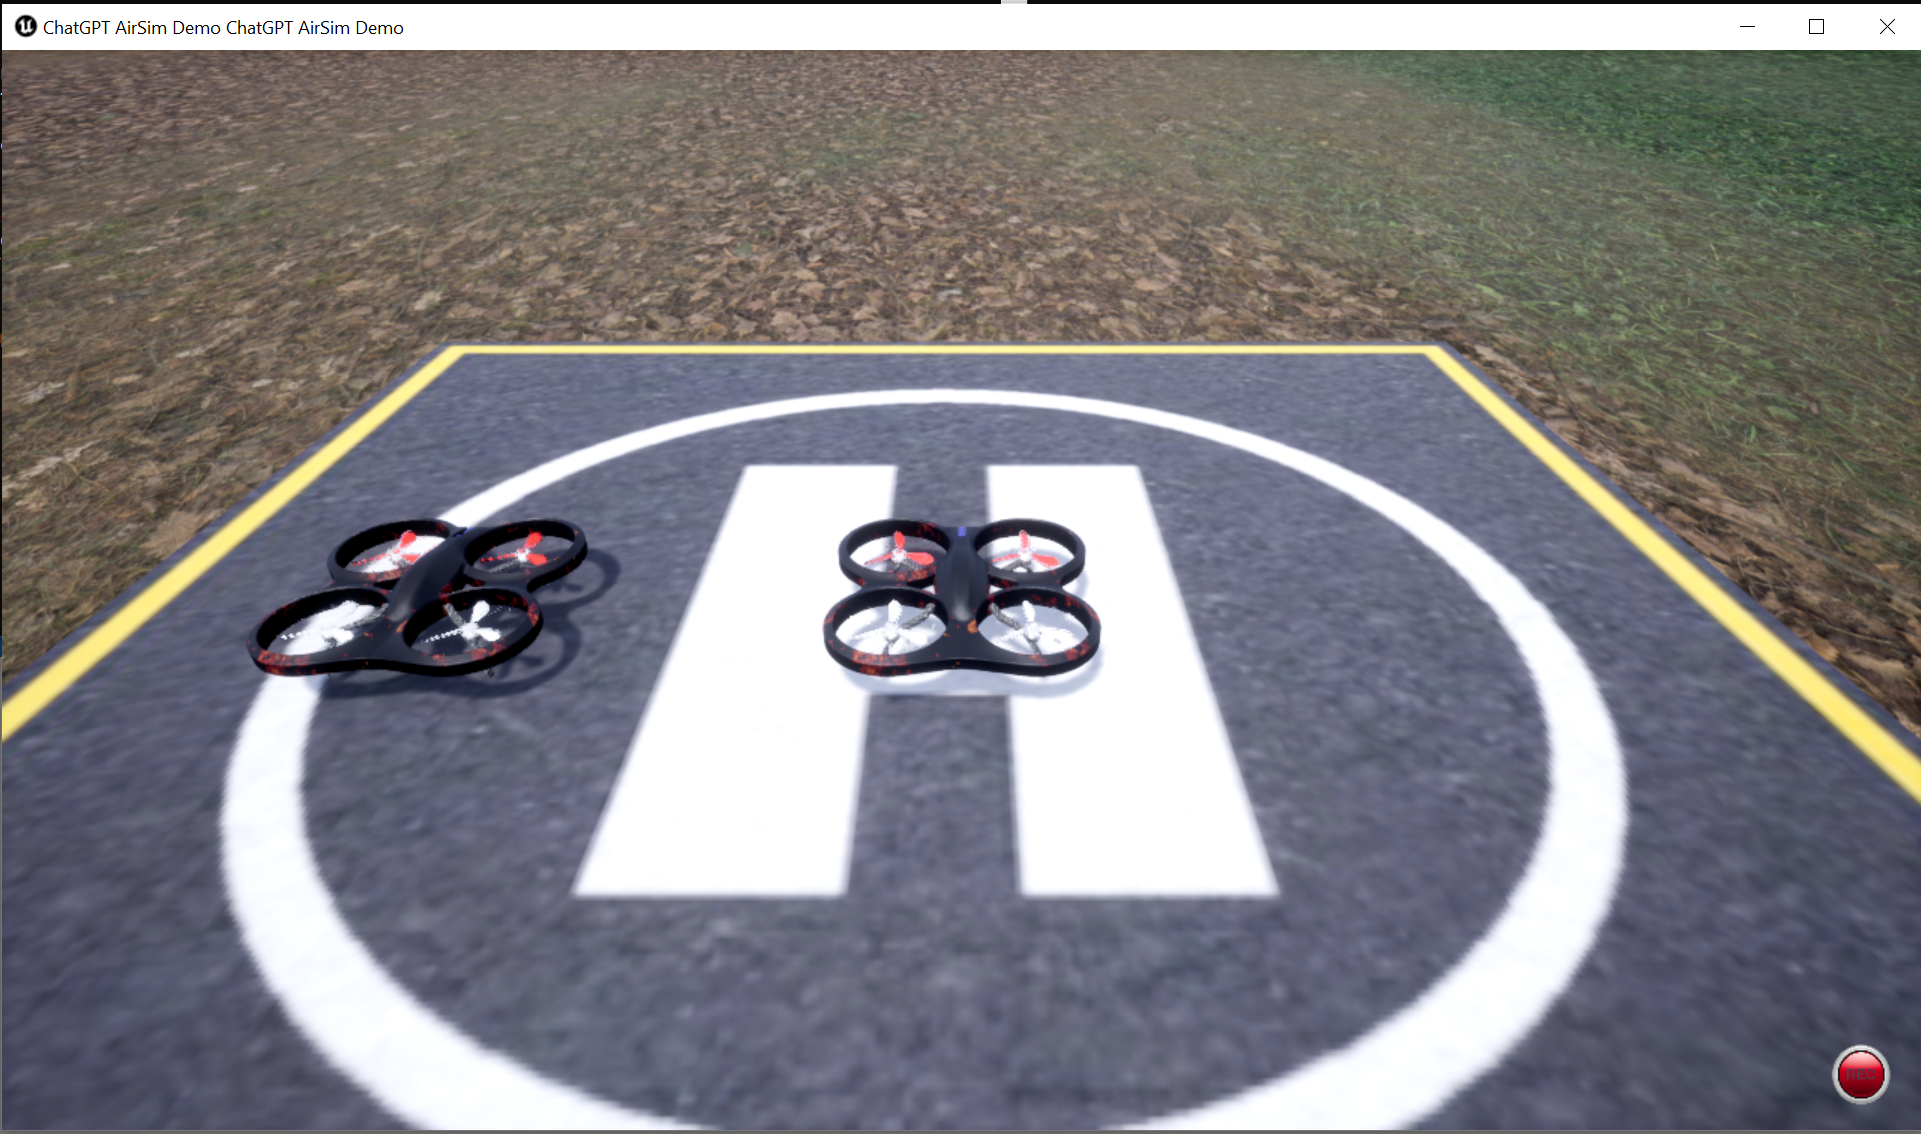
\includegraphics[width=1\linewidth]{2drones.PNG}
    \caption{Two drones on the launchpad pre takeoff}
    \label{fig:enter-label}
\end{figure}
B. Performance Metrics: We define a set of performance metrics to quantify the effectiveness and efficiency of the multi-robot coordination system. These metrics include surveillance coverage, object detection accuracy, communication latency, and resource utilization. By systematically measuring these metrics across different experimental scenarios, we can evaluate the system's capabilities and identify areas for improvement.

C. Experimental Scenarios: We design a series of experimental scenarios to evaluate the system's performance across varying levels of complexity and environmental conditions. These scenarios include static and dynamic object surveillance tasks, as well as scenarios with varying numbers of drones and surveillance objectives. By systematically varying these parameters, we can assess the system's scalability, adaptability, and robustness in real-world surveillance missions.
\begin{figure}[h]
    \centering
    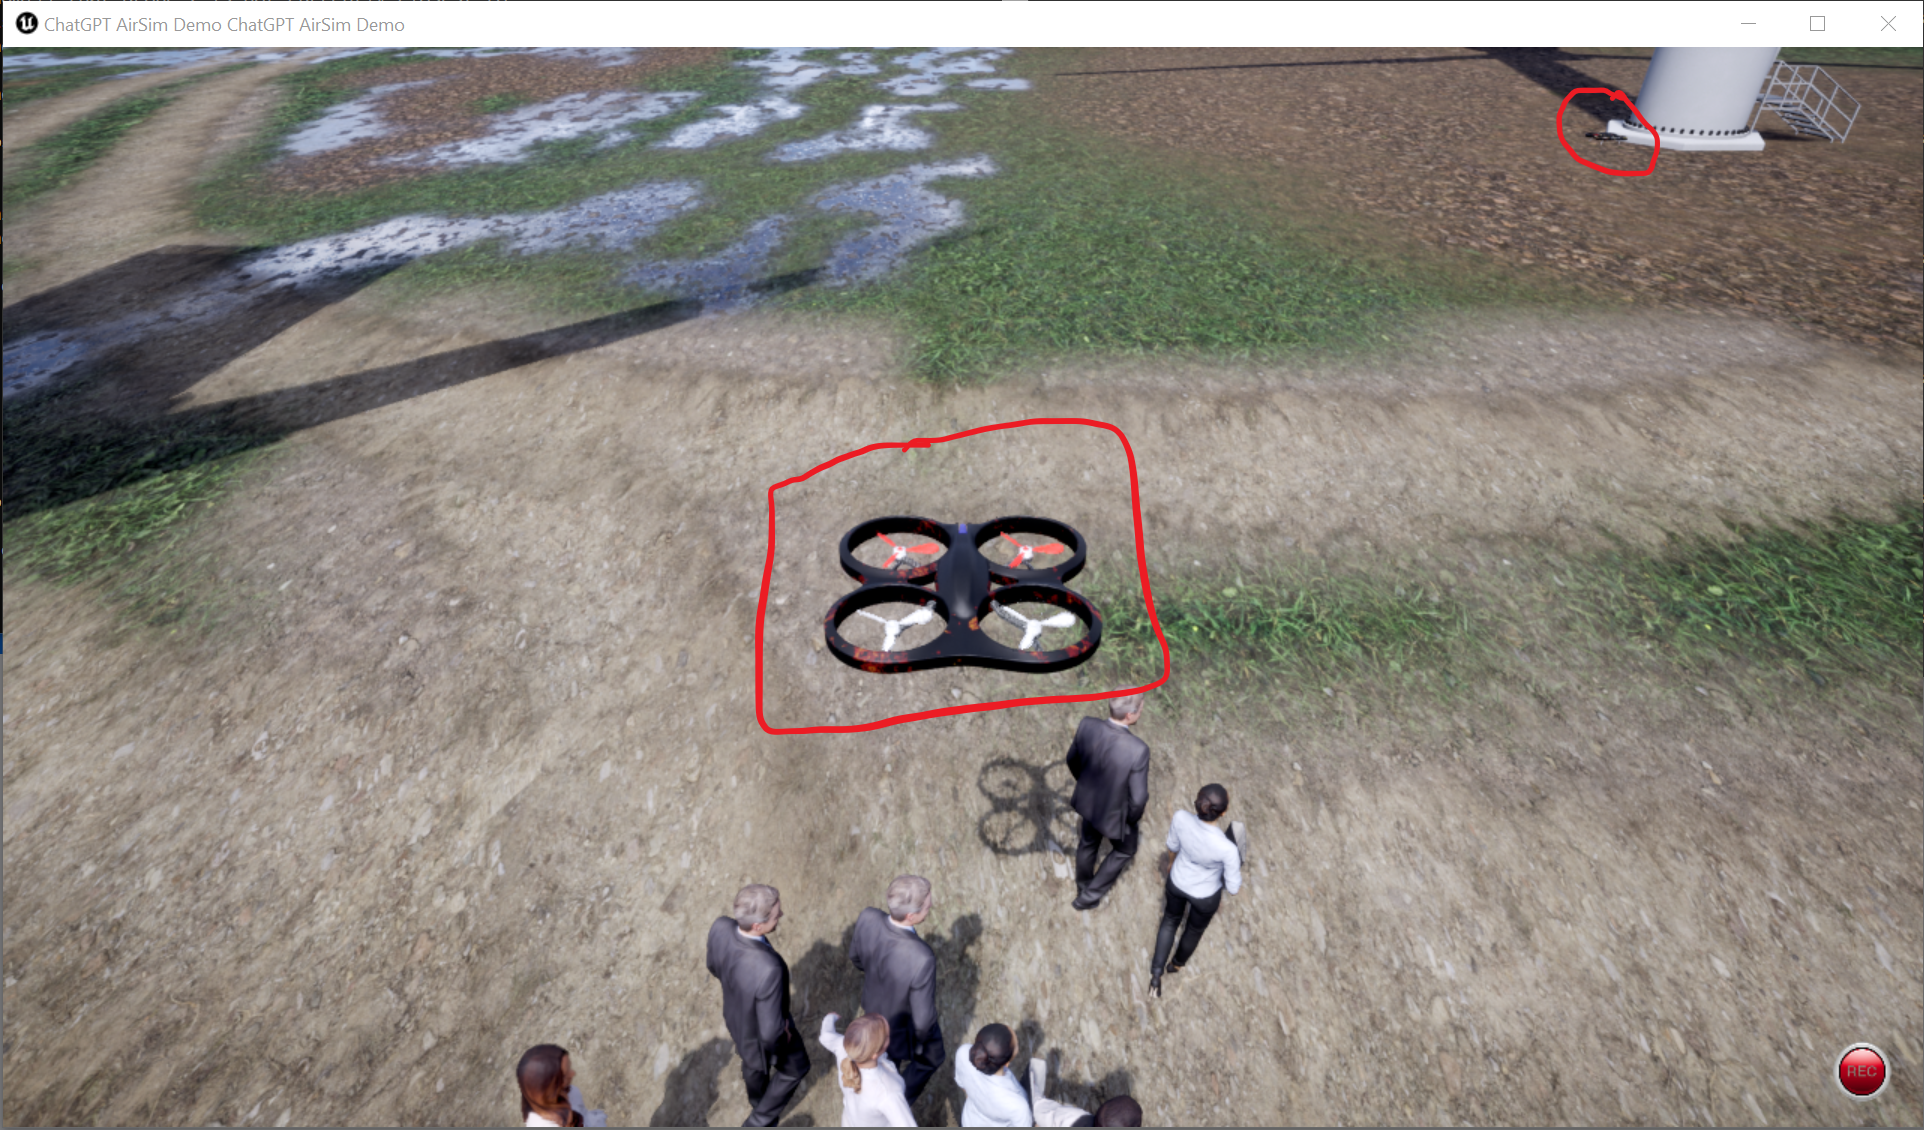
\includegraphics[width=1\linewidth]{2drones_ppl_wmd.PNG}
    \caption{Two drones, one surveying a group of people and one in the top right at the base of a windmill}
    \label{fig:enter-label}
\end{figure}
...

\section{Results and Discussion}

The results of our experimental evaluation and discuss the findings in the context of multi-robot coordination for object surveillance tasks.

A. Quantitative Analysis: We analyze the quantitative results obtained from the experimental evaluation, focusing on key performance metrics such as surveillance coverage, object detection accuracy, and communication efficiency. Our analysis reveals the system's ability to effectively coordinate multiple drones using ChatGPT, resulting in improved surveillance performance compared to traditional centralized approaches. We also discuss the impact of environmental factors and task complexity on the system's performance.

B. Qualitative Assessment: In addition to quantitative analysis, we provide a qualitative assessment of the system's behavior and performance based on observed patterns and experimental insights. We discuss the system's adaptability to dynamic changes in the surveillance environment, its ability to handle communication failures and partial observability, and its overall effectiveness in real-world surveillance missions. This qualitative assessment complements the quantitative analysis and provides valuable insights into the system's strengths and limitations.
...

\section{Potential Future Impact and Development}

Industrial robotics stands as one of the most prominent fields where the integration of Large Language Models (LLMs) like ChatGPT holds significant potential. In manufacturing automation, ChatGPT can assist in optimizing production schedules, allocating resources, and coordinating tasks within manufacturing facilities. With its ability to analyze sensor data in real-time, LLMs facilitate quality assurance by detecting defects, ensuring product quality, and minimizing waste during manufacturing processes. Moreover, industrial robots equipped with LLMs can collaborate with human workers to efficiently allocate tasks, balance workloads, and improve overall productivity. Especially with how this technology simplifies the user/robot interaction considerably, workers do not have to be fully technically skilled opening the gateway to employment to many more

Human-robot collaboration is enhanced through ChatGPT's capabilities, enabling cooperative assembly tasks where robots provide assistance, feedback, and guidance to human workers. Safety monitoring becomes more robust with LLMs analyzing sensor data to detect safety hazards, monitor interactions, and ensure safe working conditions. Skill transfer is facilitated as well, with ChatGPT capturing and codifying expert knowledge for robots to learn new tasks and adapt to changing production requirements.

Disaster response stands as a critical domain where the integration of LLMs can significantly improve preparedness, coordination, and efficiency in managing crises. In this context, ChatGPT can play a vital role in various aspects of disaster response:

During the response phase of a disaster, LLMs can assist in coordinating emergency operations, managing resources, and disseminating critical information to first responders and affected populations. ChatGPT-powered systems can analyze real-time data from sensors, social media feeds, and other sources to provide situational awareness, identify priority areas, and allocate resources effectively.

Search and rescue operations benefit from ChatGPT's ability to analyze terrain data, plan search patterns, and coordinate rescue efforts. LLMs can assist in identifying optimal search routes, prioritizing areas for search teams, and providing real-time updates on rescue operations.

In infrastructure assessment and damage evaluation, ChatGPT can analyze aerial imagery, satellite data, and sensor readings to assess the extent of damage, identify critical infrastructure failures, and prioritize repair efforts. By analyzing data from drones and other unmanned systems, LLMs can provide insights into road conditions, bridge stability, and building integrity, facilitating rapid response and recovery efforts.

One way we can develop this technology further is with implementing multiple robot control with a drone and a car instead of only multiple drones. Implementing two and upwards drones with the method we have at hand is simple and is only constrained by the hardware we are running the simulator on. If you watch the video attached to this paper, the demo of Airsim with two drones, you see that the simulator is rather slow showing the hardware constraints of the machine we ran it on. Implementing a car and a drone both as robots takes a higher level of difficulty. Integrating the car and drone environment with the ChatGPT bridge is the next step, Allowing both robots to not only move synchronously but also allow each robot to accurately track the location of each other. 



\section{Conclusion}

In this study, a new method for coordinating multiple robots in object surveillance missions has been introduced, employing ChatGPT. Through the incorporation of ChatGPT into the coordination framework, the study has showcased the system's capacity to facilitate decentralized communication, dynamic task distribution, and context-sensitive decision-making across a group of drones. The results of the experimental assessment suggest that the ChatGPT-infused system surpasses conventional centralized methods in terms of surveillance scope, object identification precision, and communication effectiveness. These outcomes underscore the promise of conversational AI models like ChatGPT in enhancing the functionalities of multi-robot systems for practical uses like object surveillance and supervision.

...
\begin{thebibliography}{1}
\bibitem{vemprala2023chatgpt}
S. Vemprala, R. Bonatti, A. Bucker, and A. Kapoor, "Chatgpt for robotics: Design principles and model abilities," Microsoft, https://www.microsoft.com/en-us/research/uploads/prod/2023/02/ChatGPTRobotics.pdf (accessed Mar. 19, 2024).

\bibitem{airsim2017fsr}
S. Shah, D. Dey, C. Lovett, and A. Kapoor, "AirSim: High-Fidelity Visual and Physical Simulation for Autonomous Vehicles," in \textit{Field and Service Robotics}, 2017, \url{https://arxiv.org/abs/1705.05065}.

\end{thebibliography}

\end{document}
